\subsubsection*{Project 3: Modeling oxygen insertion in one-dimensional channels of shafarzikite-like structures}\label{deLaune}
Recent study of schafarzikite-like (FeSb2O4) materials have been shown to store relatively large amounts of oxygen (~3.5\% mass)
within the structure at low temperatures (~350 °C) without decomposition, leading to new possibilities as potential oxygen storage materials.

\begin{wrapfigure}{r}{0.5\textwidth}
  \begin{center}
    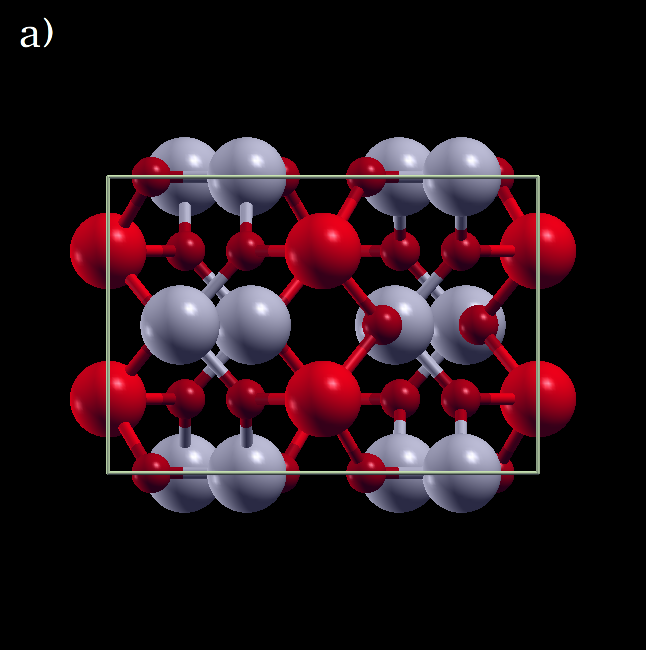
\includegraphics[width=0.24\textwidth]{graphics/fesb2o4_xaxis.png}
    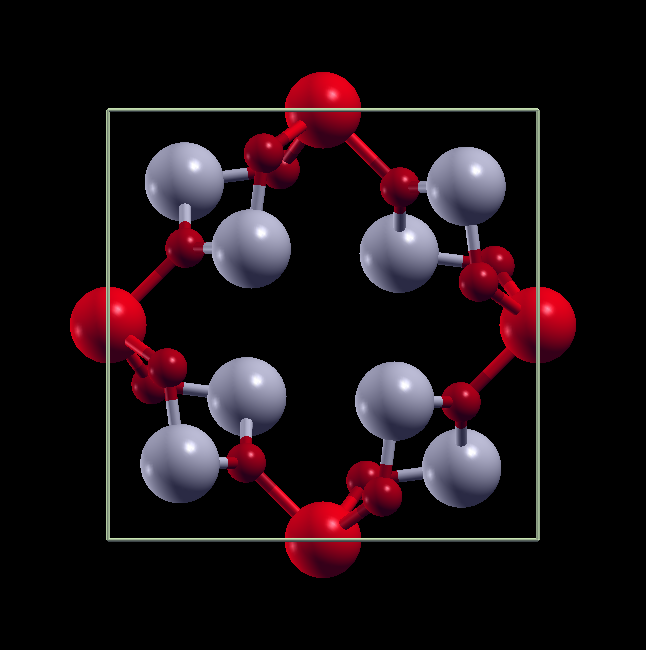
\includegraphics[width=0.24\textwidth]{graphics/fesb2o4_zaxis.png}
    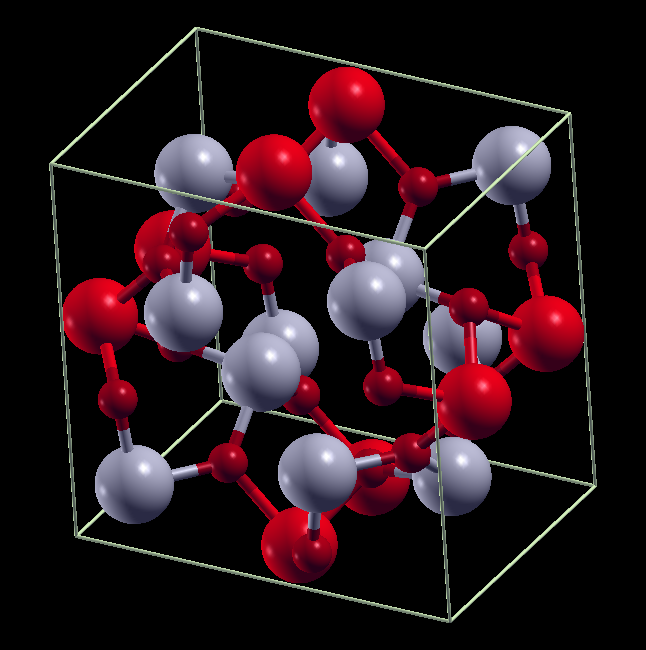
\includegraphics[width=0.38\textwidth]{graphics/fesb2o4_tilted.png}
  \end{center}
  \caption{Schafarzikite}
\end{wrapfigure} Specifically, oxygen insertion into cobalt and lead doped derivatives of shafarzikite show promise in applications of electro-catalysis due to their unique 1-D cation channels with high peroxide anion mobility and potential for high, directed electronic conductivity. We plan to analysis the neutron scattering data with RMC modeling to clarify the structures that occur before and after oxidization and also variants of the material with different doping agents. Structures generated from the RMC modeling can then be used to construct nudge elastic band calculations using density functional theory to determine transition state energy barriers during the oxidation process. Results from this study would help in clarifying the proposed defect cluster produced by the low temperature oxidation reaction.

